\documentclass[../report]{subfiles}
\setcounter{section}{0}
\begin{document}

本章では,本プロジェクトの背景と目的を説明する.
\bunseki{佐藤碧}


\section{認知症の現状}
近年の我が国では,認知症患者数が増加傾向にある.
二宮(2014)によると,2012年時点で日本国内の推定認知症患者数は462万人であった\cite{syourai}.
2025年では675万人,2040年には802万人にまで上ると予想されている(図\ref{fig:ninchisyo-graph}).
また同研究によると,65歳以上の高齢者の推定認知症有病率は2012年では15.5%,2025年には20.6%,2040年には25.4%と,年々増加していくと予想されている\cite{syourai}.
\begin{figure}[htbp]
    \begin{center}
        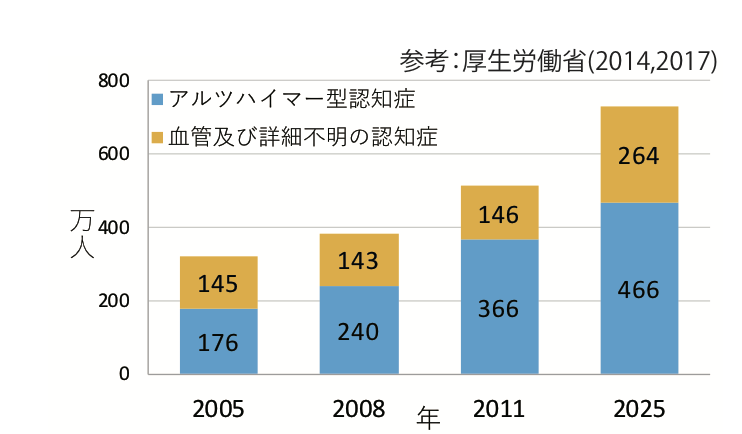
\includegraphics[width=10cm]{imgs/ninchisyo-graph.png}
        \caption{日本の認知症の総患者数の推移}
        \label{fig:ninchisyo-graph}
    \end{center}
\end{figure}
\bunseki{佐藤碧}


\section{認知症の発症原因} \label{sec:cause}
認知症は,その症状を引き起こす病気の種類によっていくつにも分類される.
例えば,「アルツハイマー病」「レビー小体型認知症」「前頭側頭型認知症」「脳血管性認知症」といったように分類される.
更に,それらの病気の原因として生活習慣病があげられる.
生活習慣病は従来より「脳血管性認知症」との関連が指摘されてきた.
だが近年の研究によって,生活習慣病は「アルツハイマー病」にも関連があり,その発症や進行に大きく関わっている事がわかってきた\cite{seikatsu}.
例えば,「高血圧」「糖尿病」「脂質異常病」といった生活習慣病が,認知症と関係のあるとされている(図\ref{fig:relation-dementia-life-habit}).
\begin{figure}[htbp]
    \begin{center}
        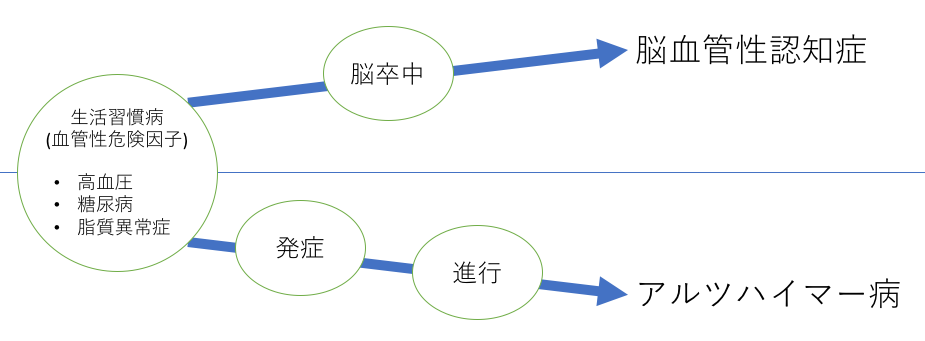
\includegraphics[width=10cm]{imgs/relation-dementia-life-habit.png}
        \caption{認知症と生活習慣病の関係}
        \label{fig:relation-dementia-life-habit}
    \end{center}
\end{figure}
\bunseki{佐藤碧}


\section{認知症と食習慣の関係}
\ref{sec:cause}でも述べたように,認知症は生活習慣病と関係がある.
「脳血管性認知症」は血管性の病気によって引き起こされる認知症である.
したがって,生活習慣病を予防して健康的な血管を維持できるようにすれば,「脳血管性認知症」の発症を抑えることが可能である.
また近年の縦断的疫学調査や5$\sim$10年にわたる大規模な追跡調査の結果では,「アルツハイマー症」には食事栄養が密接に関わっていると報告されている\cite{nutrition-dementia-00}\cite{nutrition-dementia-01}.
\bunseki{佐藤碧}


\section{認知症研究について}
認知症関係で行われている研究としては,認知症患者を対象とした認知症がもたらす問題に関する研究,認知症患者をサポートする介護者を対象とした介護の負担軽減に関する研究,認知症になる以前の人を対象とした認知症予防に関する研究に分類することができる.
認知症が原因で認知症患者が徘徊して自宅に戻れないという問題や,認知症患者数が年々増加傾向にあるということで介護者の負担が大きくなってきているという問題がある.
認知症予防の研究で「認知症の予防には,日常生活の中でコミュニケーションを充実させて脳の機能を活性化することを心がけ,食事と運動のバランスをとる生活習慣病対策を意識したライフスタイルを実践することが大切である.」\cite{dementia-prevention}ということが明らかになっている.
本グループでは,認知症になる以前の人を対象として,高齢者でも簡単に扱えるようにユーザが行う操作を最小限にして食生活を管理できるシステムの開発を行った.
\bunseki{佐藤碧}

\end{document}
